% \pdfoutput=1

\documentclass[11pt]{article}

% \usepackage[review]{ACL2023}
\usepackage{ACL2023}

\usepackage{times}
\usepackage{latexsym}
\usepackage[T1]{fontenc}
\usepackage[utf8]{inputenc}
\usepackage{microtype}
\usepackage{inconsolata}
\usepackage{hyperref}
% \RequirePackage{algorithm}
% \RequirePackage{algorithmic}

\usepackage{multirow}
\usepackage{amsmath}
\usepackage{capt-of}
\usepackage{tabularx}
% \usepackage[caption=false]{subfig}
\usepackage{subcaption}
\usepackage{epsfig}
\usepackage{amssymb}
\usepackage{amsfonts}
\usepackage{booktabs}
\usepackage{scalerel}
%\usepackage[dvipsnames]{xcolor}
\usepackage[inline]{enumitem}
\usepackage{listings}
\usepackage{varwidth}
\usepackage[export]{adjustbox}
\usepackage{tikz}
\usetikzlibrary{tikzmark}
% \usepackage{todonotes}
% \usepackage{cleveref}
\newcommand{\crefrangeconjunction}{--}
\usepackage{stmaryrd}
\usepackage{bbm}
\usepackage{wrapfig}
\usepackage{pifont}

\newcommand{\tabincell}[2]{\begin{tabular}{@{}#1@{}}#2\end{tabular}}
\newcommand{\tx}[1]{``\textit{#1}''}
\newcommand{\sptk}[1]{\texttt{[#1]}}
% \newcommand{\eqform}[1]{Equation~(\ref{#1})}

% \usepackage{algorithm}
% \usepackage[noend]{algpseudocode}

\definecolor{deepblue}{rgb}{0,0,0.5}
\definecolor{officeblue}{RGB}{0,102,204}
\definecolor{deepred}{rgb}{0.6,0,0}
\definecolor{deepgreen}{rgb}{0,0.5,0}
\definecolor{mybrickred}{RGB}{182,50,28}
\newcommand\mybox[2][]{\tikz[overlay]\node[inner sep=1pt, anchor=text, rectangle, rounded corners=0mm,#1] {#2};\phantom{#2}}
\definecolor{fillcolor}{RGB}{216,217,252}
\newcommand\bg[1]{\mybox[fill=blue!20]{#1}}
\newcommand\rg[1]{\mybox[fill=red!20]{#1}}
\newcommand\graybox[1]{\mybox[fill=gray!20]{#1}}

% %%%%%Algorithm Box Package%%%%%
% \renewcommand{\algorithmicrequire}{\textbf{Input:}}
% \algnewcommand\algorithmicrequireb{{\hspace{0.85cm}}}
% \algnewcommand\INPTDESCB{\item[\algorithmicrequireb]}
% \renewcommand{\algorithmicensure}{\textbf{Output:}}
% \algnewcommand\algorithmicfuncdesc{\textbf{Function:}}
% \algnewcommand\FUNCDESC{\item[\algorithmicfuncdesc]}
% \algnewcommand\algorithmicfuncdescb{{\hspace{1.48cm}}}
% \algnewcommand\FUNCDESCB{\item[\algorithmicfuncdescb]}
% \algnewcommand{\algorithmicgoto}{\textbf{goto}}
% \algnewcommand{\Goto}[1]{\algorithmicgoto~\ref{#1}}
% \newcommand*\Let[2]{\State {#1 $\gets$ #2}}
% \newcommand*\LineLet[2]{#1 $\gets$ #2}
% %\newcommand*\AddOne[1]{\State #1 $\gets$ #1 $+1$}
% \newcommand*\AddOne[1]{\State #1 $++$}
% \newcommand*\LineComment[1]{\Statex \(\triangleright\) #1}
% \newcommand*\LineFor[2]{\State {\algorithmicfor~#1~\algorithmicdo~~~~#2}}
% \newcommand*\LineIf[2]{\State {\algorithmicif~#1~\algorithmicthen~~~~#2}}
% \newcommand*\AlgCommentInLine[1]{{\color{deepblue}{$\triangleright$ \textit{#1}}}}
% \newcommand*\AlgComment[1]{\State{\AlgCommentInLine{#1}}}
% %%%%%Algorithm Box Package%%%%%

\newcommand*\AlgCommentInLine[1]{{\color{deepblue}{$\triangleright$ \textit{#1}}}}

%%%%% NEW MATH DEFINITIONS %%%%%

\usepackage{amsmath,amsfonts,bm}

\newcommand\sizeof[1]{\left|#1\right|}

% Mark sections of captions for referring to divisions of figures
\newcommand{\figleft}{{\em (Left)}}
\newcommand{\figcenter}{{\em (Center)}}
\newcommand{\figright}{{\em (Right)}}
\newcommand{\figtop}{{\em (Top)}}
\newcommand{\figbottom}{{\em (Bottom)}}
\newcommand{\captiona}{{\em (a)}}
\newcommand{\captionb}{{\em (b)}}
\newcommand{\captionc}{{\em (c)}}
\newcommand{\captiond}{{\em (d)}}

% Highlight a newly defined term
\newcommand{\newterm}[1]{{\bf #1}}


% Figure reference, lower-case.
\def\figref#1{figure~\ref{#1}}
% Figure reference, capital. For start of sentence
\def\Figref#1{Figure~\ref{#1}}
\def\twofigref#1#2{figures \ref{#1} and \ref{#2}}
\def\quadfigref#1#2#3#4{figures \ref{#1}, \ref{#2}, \ref{#3} and \ref{#4}}
% Section reference, lower-case.
\def\secref#1{section~\ref{#1}}
% Section reference, capital.
\def\Secref#1{Section~\ref{#1}}
% Reference to two sections.
\def\twosecrefs#1#2{sections \ref{#1} and \ref{#2}}
% Reference to three sections.
\def\secrefs#1#2#3{sections \ref{#1}, \ref{#2} and \ref{#3}}
% Reference to an equation, lower-case.
\def\eqref#1{equation~\ref{#1}}
% Reference to an equation, upper case
\def\Eqref#1{Equation~\ref{#1}}
% A raw reference to an equation---avoid using if possible
\def\plaineqref#1{\ref{#1}}
% Reference to a chapter, lower-case.
\def\chapref#1{chapter~\ref{#1}}
% Reference to an equation, upper case.
\def\Chapref#1{Chapter~\ref{#1}}
% Reference to a range of chapters
\def\rangechapref#1#2{chapters\ref{#1}--\ref{#2}}
% Reference to an algorithm, lower-case.
\def\algref#1{algorithm~\ref{#1}}
% Reference to an algorithm, upper case.
\def\Algref#1{Algorithm~\ref{#1}}
\def\twoalgref#1#2{algorithms \ref{#1} and \ref{#2}}
\def\Twoalgref#1#2{Algorithms \ref{#1} and \ref{#2}}
% Reference to a part, lower case
\def\partref#1{part~\ref{#1}}
% Reference to a part, upper case
\def\Partref#1{Part~\ref{#1}}
\def\twopartref#1#2{parts \ref{#1} and \ref{#2}}

\def\ceil#1{\lceil #1 \rceil}
\def\floor#1{\lfloor #1 \rfloor}
\def\1{\bm{1}}
\newcommand{\train}{\mathcal{D}}
\newcommand{\valid}{\mathcal{D_{\mathrm{valid}}}}
\newcommand{\test}{\mathcal{D_{\mathrm{test}}}}

\def\eps{{\epsilon}}


% Random variables
\def\reta{{\textnormal{$\eta$}}}
\def\ra{{\textnormal{a}}}
\def\rb{{\textnormal{b}}}
\def\rc{{\textnormal{c}}}
\def\rd{{\textnormal{d}}}
\def\re{{\textnormal{e}}}
\def\rf{{\textnormal{f}}}
\def\rg{{\textnormal{g}}}
\def\rh{{\textnormal{h}}}
\def\ri{{\textnormal{i}}}
\def\rj{{\textnormal{j}}}
\def\rk{{\textnormal{k}}}
\def\rl{{\textnormal{l}}}
% rm is already a command, just don't name any random variables m
\def\rn{{\textnormal{n}}}
\def\ro{{\textnormal{o}}}
\def\rp{{\textnormal{p}}}
\def\rq{{\textnormal{q}}}
\def\rr{{\textnormal{r}}}
\def\rs{{\textnormal{s}}}
\def\rt{{\textnormal{t}}}
\def\ru{{\textnormal{u}}}
\def\rv{{\textnormal{v}}}
\def\rw{{\textnormal{w}}}
\def\rx{{\textnormal{x}}}
\def\ry{{\textnormal{y}}}
\def\rz{{\textnormal{z}}}

% Random vectors
\def\rvepsilon{{\mathbf{\epsilon}}}
\def\rvtheta{{\mathbf{\theta}}}
\def\rva{{\mathbf{a}}}
\def\rvb{{\mathbf{b}}}
\def\rvc{{\mathbf{c}}}
\def\rvd{{\mathbf{d}}}
\def\rve{{\mathbf{e}}}
\def\rvf{{\mathbf{f}}}
\def\rvg{{\mathbf{g}}}
\def\rvh{{\mathbf{h}}}
\def\rvu{{\mathbf{i}}}
\def\rvj{{\mathbf{j}}}
\def\rvk{{\mathbf{k}}}
\def\rvl{{\mathbf{l}}}
\def\rvm{{\mathbf{m}}}
\def\rvn{{\mathbf{n}}}
\def\rvo{{\mathbf{o}}}
\def\rvp{{\mathbf{p}}}
\def\rvq{{\mathbf{q}}}
\def\rvr{{\mathbf{r}}}
\def\rvs{{\mathbf{s}}}
\def\rvt{{\mathbf{t}}}
\def\rvu{{\mathbf{u}}}
\def\rvv{{\mathbf{v}}}
\def\rvw{{\mathbf{w}}}
\def\rvx{{\mathbf{x}}}
\def\rvy{{\mathbf{y}}}
\def\rvz{{\mathbf{z}}}

% Elements of random vectors
\def\erva{{\textnormal{a}}}
\def\ervb{{\textnormal{b}}}
\def\ervc{{\textnormal{c}}}
\def\ervd{{\textnormal{d}}}
\def\erve{{\textnormal{e}}}
\def\ervf{{\textnormal{f}}}
\def\ervg{{\textnormal{g}}}
\def\ervh{{\textnormal{h}}}
\def\ervi{{\textnormal{i}}}
\def\ervj{{\textnormal{j}}}
\def\ervk{{\textnormal{k}}}
\def\ervl{{\textnormal{l}}}
\def\ervm{{\textnormal{m}}}
\def\ervn{{\textnormal{n}}}
\def\ervo{{\textnormal{o}}}
\def\ervp{{\textnormal{p}}}
\def\ervq{{\textnormal{q}}}
\def\ervr{{\textnormal{r}}}
\def\ervs{{\textnormal{s}}}
\def\ervt{{\textnormal{t}}}
\def\ervu{{\textnormal{u}}}
\def\ervv{{\textnormal{v}}}
\def\ervw{{\textnormal{w}}}
\def\ervx{{\textnormal{x}}}
\def\ervy{{\textnormal{y}}}
\def\ervz{{\textnormal{z}}}

% Random matrices
\def\rmA{{\mathbf{A}}}
\def\rmB{{\mathbf{B}}}
\def\rmC{{\mathbf{C}}}
\def\rmD{{\mathbf{D}}}
\def\rmE{{\mathbf{E}}}
\def\rmF{{\mathbf{F}}}
\def\rmG{{\mathbf{G}}}
\def\rmH{{\mathbf{H}}}
\def\rmI{{\mathbf{I}}}
\def\rmJ{{\mathbf{J}}}
\def\rmK{{\mathbf{K}}}
\def\rmL{{\mathbf{L}}}
\def\rmM{{\mathbf{M}}}
\def\rmN{{\mathbf{N}}}
\def\rmO{{\mathbf{O}}}
\def\rmP{{\mathbf{P}}}
\def\rmQ{{\mathbf{Q}}}
\def\rmR{{\mathbf{R}}}
\def\rmS{{\mathbf{S}}}
\def\rmT{{\mathbf{T}}}
\def\rmU{{\mathbf{U}}}
\def\rmV{{\mathbf{V}}}
\def\rmW{{\mathbf{W}}}
\def\rmX{{\mathbf{X}}}
\def\rmY{{\mathbf{Y}}}
\def\rmZ{{\mathbf{Z}}}

% Elements of random matrices
\def\ermA{{\textnormal{A}}}
\def\ermB{{\textnormal{B}}}
\def\ermC{{\textnormal{C}}}
\def\ermD{{\textnormal{D}}}
\def\ermE{{\textnormal{E}}}
\def\ermF{{\textnormal{F}}}
\def\ermG{{\textnormal{G}}}
\def\ermH{{\textnormal{H}}}
\def\ermI{{\textnormal{I}}}
\def\ermJ{{\textnormal{J}}}
\def\ermK{{\textnormal{K}}}
\def\ermL{{\textnormal{L}}}
\def\ermM{{\textnormal{M}}}
\def\ermN{{\textnormal{N}}}
\def\ermO{{\textnormal{O}}}
\def\ermP{{\textnormal{P}}}
\def\ermQ{{\textnormal{Q}}}
\def\ermR{{\textnormal{R}}}
\def\ermS{{\textnormal{S}}}
\def\ermT{{\textnormal{T}}}
\def\ermU{{\textnormal{U}}}
\def\ermV{{\textnormal{V}}}
\def\ermW{{\textnormal{W}}}
\def\ermX{{\textnormal{X}}}
\def\ermY{{\textnormal{Y}}}
\def\ermZ{{\textnormal{Z}}}

% Vectors
\def\vzero{{\bm{0}}}
\def\vone{{\bm{1}}}
\def\vmu{{\bm{\mu}}}
\def\vtheta{{\bm{\theta}}}
\def\va{{\bm{a}}}
\def\vb{{\bm{b}}}
\def\vc{{\bm{c}}}
\def\vd{{\bm{d}}}
\def\ve{{\bm{e}}}
\def\vf{{\bm{f}}}
\def\vg{{\bm{g}}}
\def\vh{{\bm{h}}}
\def\vi{{\bm{i}}}
\def\vj{{\bm{j}}}
\def\vk{{\bm{k}}}
\def\vl{{\bm{l}}}
\def\vm{{\bm{m}}}
\def\vn{{\bm{n}}}
\def\vo{{\bm{o}}}
\def\vp{{\bm{p}}}
\def\vq{{\bm{q}}}
\def\vr{{\bm{r}}}
\def\vs{{\bm{s}}}
\def\vt{{\bm{t}}}
\def\vu{{\bm{u}}}
\def\vv{{\bm{v}}}
\def\vw{{\bm{w}}}
\def\vx{{\bm{x}}}
\def\vy{{\bm{y}}}
\def\vz{{\bm{z}}}

% Elements of vectors
\def\evalpha{{\alpha}}
\def\evbeta{{\beta}}
\def\evepsilon{{\epsilon}}
\def\evlambda{{\lambda}}
\def\evomega{{\omega}}
\def\evmu{{\mu}}
\def\evpsi{{\psi}}
\def\evsigma{{\sigma}}
\def\evtheta{{\theta}}
\def\eva{{a}}
\def\evb{{b}}
\def\evc{{c}}
\def\evd{{d}}
\def\eve{{e}}
\def\evf{{f}}
\def\evg{{g}}
\def\evh{{h}}
\def\evi{{i}}
\def\evj{{j}}
\def\evk{{k}}
\def\evl{{l}}
\def\evm{{m}}
\def\evn{{n}}
\def\evo{{o}}
\def\evp{{p}}
\def\evq{{q}}
\def\evr{{r}}
\def\evs{{s}}
\def\evt{{t}}
\def\evu{{u}}
\def\evv{{v}}
\def\evw{{w}}
\def\evx{{x}}
\def\evy{{y}}
\def\evz{{z}}

% Matrix
\def\mA{{\bm{A}}}
\def\mB{{\bm{B}}}
\def\mC{{\bm{C}}}
\def\mD{{\bm{D}}}
\def\mE{{\bm{E}}}
\def\mF{{\bm{F}}}
\def\mG{{\bm{G}}}
\def\mH{{\bm{H}}}
\def\mI{{\bm{I}}}
\def\mJ{{\bm{J}}}
\def\mK{{\bm{K}}}
\def\mL{{\bm{L}}}
\def\mM{{\bm{M}}}
\def\mN{{\bm{N}}}
\def\mO{{\bm{O}}}
\def\mP{{\bm{P}}}
\def\mQ{{\bm{Q}}}
\def\mR{{\bm{R}}}
\def\mS{{\bm{S}}}
\def\mT{{\bm{T}}}
\def\mU{{\bm{U}}}
\def\mV{{\bm{V}}}
\def\mW{{\bm{W}}}
\def\mX{{\bm{X}}}
\def\mY{{\bm{Y}}}
\def\mZ{{\bm{Z}}}
\def\mBeta{{\bm{\beta}}}
\def\mPhi{{\bm{\Phi}}}
\def\mLambda{{\bm{\Lambda}}}
\def\mSigma{{\bm{\Sigma}}}

% Tensor
\DeclareMathAlphabet{\mathsfit}{\encodingdefault}{\sfdefault}{m}{sl}
\SetMathAlphabet{\mathsfit}{bold}{\encodingdefault}{\sfdefault}{bx}{n}
\newcommand{\tens}[1]{\bm{\mathsfit{#1}}}
\def\tA{{\tens{A}}}
\def\tB{{\tens{B}}}
\def\tC{{\tens{C}}}
\def\tD{{\tens{D}}}
\def\tE{{\tens{E}}}
\def\tF{{\tens{F}}}
\def\tG{{\tens{G}}}
\def\tH{{\tens{H}}}
\def\tI{{\tens{I}}}
\def\tJ{{\tens{J}}}
\def\tK{{\tens{K}}}
\def\tL{{\tens{L}}}
\def\tM{{\tens{M}}}
\def\tN{{\tens{N}}}
\def\tO{{\tens{O}}}
\def\tP{{\tens{P}}}
\def\tQ{{\tens{Q}}}
\def\tR{{\tens{R}}}
\def\tS{{\tens{S}}}
\def\tT{{\tens{T}}}
\def\tU{{\tens{U}}}
\def\tV{{\tens{V}}}
\def\tW{{\tens{W}}}
\def\tX{{\tens{X}}}
\def\tY{{\tens{Y}}}
\def\tZ{{\tens{Z}}}


% Graph
\def\gA{{\mathcal{A}}}
\def\gB{{\mathcal{B}}}
\def\gC{{\mathcal{C}}}
\def\gD{{\mathcal{D}}}
\def\gE{{\mathcal{E}}}
\def\gF{{\mathcal{F}}}
\def\gG{{\mathcal{G}}}
\def\gH{{\mathcal{H}}}
\def\gI{{\mathcal{I}}}
\def\gJ{{\mathcal{J}}}
\def\gK{{\mathcal{K}}}
\def\gL{{\mathcal{L}}}
\def\gM{{\mathcal{M}}}
\def\gN{{\mathcal{N}}}
\def\gO{{\mathcal{O}}}
\def\gP{{\mathcal{P}}}
\def\gQ{{\mathcal{Q}}}
\def\gR{{\mathcal{R}}}
\def\gS{{\mathcal{S}}}
\def\gT{{\mathcal{T}}}
\def\gU{{\mathcal{U}}}
\def\gV{{\mathcal{V}}}
\def\gW{{\mathcal{W}}}
\def\gX{{\mathcal{X}}}
\def\gY{{\mathcal{Y}}}
\def\gZ{{\mathcal{Z}}}

% Sets
\def\sA{{\mathbb{A}}}
\def\sB{{\mathbb{B}}}
\def\sC{{\mathbb{C}}}
\def\sD{{\mathbb{D}}}
% Don't use a set called E, because this would be the same as our symbol
% for expectation.
\def\sF{{\mathbb{F}}}
\def\sG{{\mathbb{G}}}
\def\sH{{\mathbb{H}}}
\def\sI{{\mathbb{I}}}
\def\sJ{{\mathbb{J}}}
\def\sK{{\mathbb{K}}}
\def\sL{{\mathbb{L}}}
\def\sM{{\mathbb{M}}}
\def\sN{{\mathbb{N}}}
\def\sO{{\mathbb{O}}}
\def\sP{{\mathbb{P}}}
\def\sQ{{\mathbb{Q}}}
\def\sR{{\mathbb{R}}}
\def\sS{{\mathbb{S}}}
\def\sT{{\mathbb{T}}}
\def\sU{{\mathbb{U}}}
\def\sV{{\mathbb{V}}}
\def\sW{{\mathbb{W}}}
\def\sX{{\mathbb{X}}}
\def\sY{{\mathbb{Y}}}
\def\sZ{{\mathbb{Z}}}

% Entries of a matrix
\def\emLambda{{\Lambda}}
\def\emA{{A}}
\def\emB{{B}}
\def\emC{{C}}
\def\emD{{D}}
\def\emE{{E}}
\def\emF{{F}}
\def\emG{{G}}
\def\emH{{H}}
\def\emI{{I}}
\def\emJ{{J}}
\def\emK{{K}}
\def\emL{{L}}
\def\emM{{M}}
\def\emN{{N}}
\def\emO{{O}}
\def\emP{{P}}
\def\emQ{{Q}}
\def\emR{{R}}
\def\emS{{S}}
\def\emT{{T}}
\def\emU{{U}}
\def\emV{{V}}
\def\emW{{W}}
\def\emX{{X}}
\def\emY{{Y}}
\def\emZ{{Z}}
\def\emSigma{{\Sigma}}

% entries of a tensor
% Same font as tensor, without \bm wrapper
\newcommand{\etens}[1]{\mathsfit{#1}}
\def\etLambda{{\etens{\Lambda}}}
\def\etA{{\etens{A}}}
\def\etB{{\etens{B}}}
\def\etC{{\etens{C}}}
\def\etD{{\etens{D}}}
\def\etE{{\etens{E}}}
\def\etF{{\etens{F}}}
\def\etG{{\etens{G}}}
\def\etH{{\etens{H}}}
\def\etI{{\etens{I}}}
\def\etJ{{\etens{J}}}
\def\etK{{\etens{K}}}
\def\etL{{\etens{L}}}
\def\etM{{\etens{M}}}
\def\etN{{\etens{N}}}
\def\etO{{\etens{O}}}
\def\etP{{\etens{P}}}
\def\etQ{{\etens{Q}}}
\def\etR{{\etens{R}}}
\def\etS{{\etens{S}}}
\def\etT{{\etens{T}}}
\def\etU{{\etens{U}}}
\def\etV{{\etens{V}}}
\def\etW{{\etens{W}}}
\def\etX{{\etens{X}}}
\def\etY{{\etens{Y}}}
\def\etZ{{\etens{Z}}}

% The true underlying data generating distribution
\newcommand{\pdata}{p_{\rm{data}}}
% The empirical distribution defined by the training set
\newcommand{\ptrain}{\hat{p}_{\rm{data}}}
\newcommand{\Ptrain}{\hat{P}_{\rm{data}}}
% The model distribution
\newcommand{\pmodel}{p_{\rm{model}}}
\newcommand{\Pmodel}{P_{\rm{model}}}
\newcommand{\ptildemodel}{\tilde{p}_{\rm{model}}}
% Stochastic autoencoder distributions
\newcommand{\pencode}{p_{\rm{encoder}}}
\newcommand{\pdecode}{p_{\rm{decoder}}}
\newcommand{\precons}{p_{\rm{reconstruct}}}

\newcommand{\laplace}{\mathrm{Laplace}} % Laplace distribution

\newcommand{\E}{\mathbb{E}}
\newcommand{\Ls}{\mathcal{L}}
\newcommand{\R}{\mathbb{R}}
\newcommand{\emp}{\tilde{p}}
\newcommand{\lr}{\alpha}
\newcommand{\reg}{\lambda}
\newcommand{\rect}{\mathrm{rectifier}}
\newcommand{\softmax}{\mathrm{softmax}}
\newcommand{\sigmoid}{\sigma}
\newcommand{\softplus}{\zeta}
\newcommand{\KL}{D_{\mathrm{KL}}}
\newcommand{\Var}{\mathrm{Var}}
\newcommand{\standarderror}{\mathrm{SE}}
\newcommand{\Cov}{\mathrm{Cov}}
\newcommand{\diag}{\mathrm{diag}}
% Wolfram Mathworld says $L^2$ is for function spaces and $\ell^2$ is for vectors
% But then they seem to use $L^2$ for vectors throughout the site, and so does
% wikipedia.
\newcommand{\normlzero}{L^0}
\newcommand{\normlone}{L^1}
\newcommand{\normltwo}{L^2}
\newcommand{\normlp}{L^p}
\newcommand{\normmax}{L^\infty}

\newcommand{\parents}{Pa} % See usage in notation.tex. Chosen to match Daphne's book.

\DeclareMathOperator*{\argmax}{arg\,max}
\DeclareMathOperator*{\argmin}{arg\,min}

\DeclareMathOperator{\sign}{sign}
\DeclareMathOperator{\Tr}{Tr}
\let\ab\allowbreak


% \newcommand{\cmark}{\ding{51}\xspace}%
\newcommand{\cmarkg}{\textcolor{lightgray}{\ding{51}}\xspace}%
% \newcommand{\xmark}{\ding{55}\xspace}%
\newcommand{\xmarkg}{\textcolor{lightgray}{\ding{55}}\xspace}%

\newcommand\our{\textsc{structured prompting}}
\newcommand{\tblidx}[1]{{\scriptsize \texttt{[#1]}}}
\newtheorem{theorem}{Property}

\usepackage{pifont}% http://ctan.org/pkg/pifont
\newcommand{\cmark}{{\color{blue}\ding{51}}}%
\newcommand{\xmark}{{\color{black}\ding{55}}}%


\title{Understanding In-Context Learning in Large Language Models as Gradient Descent Revisted}


\newcommand*\samethanks[1][\value{footnote}]{\footnotemark[#1]}

\author{\\
Tomer Bar Natan,~Gilad Deutch,~Nadav Magar\\
~~~~Supervised by Guy Dar\\
~~~~~Tel-Aviv University}

\date{}

\begin{document}

\maketitle

\begin{abstract}
	In-context learning (ICL) has shown impressive results in few-shot learning tasks, yet the underlying mechanism of it is still not fully understood.
	Recent research suggests that ICL is similar to gradient descent (GD)-based fine-tuning.
	Mathematical analysis shows an equivalence between ICL to gradient descent on a transformer with linear attention and one layer,
	yet empirical research has shown only limited success in showing equivalence on non-linear, multi-layered models.
	In this work, we experiment with a new training process that we call per-layer training,
	and provide some empricial evidence to suggest that this process may explain the underlying mechanism of ICL better than standard fine-tuning.
	Per-layer training, we beileve, aligns better with the mathematical analysis of the ICL and GD equivalence.
	We also experiment with fine-tuning the model with linear approximation of it.
	% [git]
	Code implementation for all our experiments can be found here:
	\href{https://github.com/GiilDe/ft-vs-icl}{https://github.com/GiilDe/ft-vs-icl}
\end{abstract}

\section{Introduction}
In recent studies \cite{pmlr-v202-von-oswald23a,dai2023gpt}, attempts have been made to establish a link between in-context learning (ICL) and the fine-tuning process using gradient descent (GD) in transformer models. One common conclusion that researchers frequently derive from these studies is that "ICL essentially enacts gradient descent." Nevertheless, it's worth noting that much of the analysis in these investigations focused on models with linear attention, which can be considered as a simplified setting.

In their study, \cite{dai2023gpt} expand their findings from linear attention to conventional attention mechanisms, relying on empirical evidence to support their assertions.
Their experiments convincingly demonstrate that a model fine-tuned through gradient descent steps and a model prompted with in-context examples appear to execute similar functions. In simpler terms, they exhibit analogous behaviors when processing inputs. Furthermore, they observe a substantial overlap in the internal behaviors of these two models.
Yet, it remains unclear how a transformer's forward pass calculates its backward pass, even if it's done in a clever way involving a smaller transformer embedded within the weights of the original transformer, as suggested by some. Even if this is theoretically achievable, it's a complex concept to put into practice. In contrast, when it comes to linear models, the gradient step has a straightforward mathematical formula, making it much simpler to handle.

In \cite{pmlr-v202-von-oswald23a}, they put forth a less ambitious idea. They suggest that the model essentially carries out a kind of gradient descent on a simple linear model applied to the original deep representations calculated during the forward pass.
Using linear models with detailed feature representations is known to be highly effective in accomplishing various tasks.


In this study, our goal is to demonstrate that this principle holds true in this context as well. This can support our argument that extensive fine-tuning is not required, and a basic linear model that uses the original hidden states as inputs suffices.
To do so, we perform three experiments:
\begin{itemize}
    \item \textbf{Linearization}: We replicated the similarities results of \cite{dai2023gpt} and compared them with a simplified version the function we optimize by linearization.
    \item \textbf{Gilad's experiment}: \textbf{TODO!!}
    \item \textbf{Labels Switching}: To further confirm the results of \cite{dai2023gpt}, motivated by textbf{TODO: add relevant labels experiments papers}, we evaluated the change in similarity when providing false labels both in FT and ICL.
\end{itemize}


\section{Background and Preliminaries}
\subsection{Dual Form Between Attention and Linear Layers Optimized by Gradient Descent}

The view of language models as meta-optimizers originates from the presentation of the dual and primal forms of the perceptron \cite{Aizerman2019TheoreticalFO}.
This notion was later expressed in terms key/value/query-attention operation by by \cite{irie22dual,dai2023gpt,pmlr-v202-von-oswald23a} which apply it apply it in the modern context of deep neural networks.
They show that linear layers optimized by gradient descent have a dual representation as linear attention.

Let $W \in \mathbb{R}^{d_{\text{out}} \times d_{\text{in}}}$ be the weight matrix of a linear layer initialized at $W_0$, and let $\mathbf{x}, \mathbf{x}_1, \dots, \mathbf{x}_n  \in \mathbb{R}^{d_{\text{in}}}$ be the input and training examples representation respectively.
One step of gradient descent on the loss function $\mathcal{L}$ with learning rate $\eta$ yields the weight update $\Delta W$.
This update can be written as the outer products of the training examples $\mathbf{x}_1, \dots, \mathbf{x}_n$ and the gradients of their corresponding outputs $\mathbf{e}_i = -\eta \nabla_{W_0 x_i}\mathcal{L}$
\begin{equation}
    \Delta W = \sum_i \mathbf{e}_i \otimes \mathbf{x}^{\prime T}_i.
    \label{equ:dual_comp_2}
\end{equation}

Thus the computation of the optimized linear layer can be formulated as 

\begin{equation}
    \begin{aligned}
        \mathcal{F}(\mathbf{x}) = & \left( W_{0} + \Delta W \right) \mathbf{x} \\
        = & W_{0} \mathbf{x} + \Delta W \mathbf{x} \\
        = & W_{0} \mathbf{x} + \sum_i \left( \mathbf{e}_i \otimes \mathbf{x}_i\right) \mathbf{x} \\
        = & W_{0} \mathbf{x} + \sum_i \mathbf{e}_i \left( \mathbf{x}^{T}_i \mathbf{x} \right) \\
        = & W_{0} \mathbf{x} + \operatorname{LinearAttn} \left( E, X, \mathbf{x} \right), 
    \end{aligned}
    \label{equ:sgd_attn_dual}
\end{equation}
where $\operatorname{LinearAttn}(V, K, \mathbf{q})$ denotes the linear attention operation.
From the perspective of attention we regard training examples $X$ as keys, their corresponding gradients as values, and the current input $\mathbf{x}$ as the query.


\subsection{Understanding Transformer Attention as Meta-Optimization}
\label{sec:icl_dual}
In this section we explain the simplified mathematical view of in-context learning as a process of meta-optimization presented in \cite{dai2023gpt}.
For the purpose of analysis, it is useful to view the change to the output induced by attention to the demonstration tokens as equivalent parameter update $\Delta W_{\text{ICL}}$ that take effect on the original attention parameters.

Let $\mathbf{x} \in \mathbb{R}^{d}$ be the input representation of a query token $t$, and $\mathbf{q} = W_{Q} \mathbf{x} \in \mathbb{R}^{d^{\prime}}$ be the attention query vector. 
We use the relaxed linear attention model, whereby the softmax operation and the scaling factor are omitted:
\begin{equation}
    \begin{aligned}
    \mathcal{F}_{\text{ICL}}(\mathbf{q}) & = \operatorname{LinearAttn}(V, K, \mathbf{q}) \\
    & = W_{V} [X^{\prime}; X] \left( W_{K} [X^{\prime}; X] \right)^T \mathbf{q} \\
    \end{aligned}
    \label{equ:icl_attn}
\end{equation}
where $W_{Q}, W_{K}, W_{V} \in \mathbb{R}^{d^{\prime} \times d}$ are the projection matrices for computing the attention queries, keys, and values, respectively; 
$X$ denotes the input representations of query tokens before $t$; 
$X^{\prime}$ denotes the input representations of the demonstration tokens; 
and $[X^{\prime}; X]$ denotes the matrix concatenation. 


They define $W_{\text{ZSL}} = W_{V} X \left( W_{K} X \right)^T$ as the initial parameters of a linear layer that is updated by attention to in-context demonstrations.
To see this, note that $W_{\text{ZSL}}$ is the attention result in the zero-shot learning setting where no demonstrations are given (Equation \ref{equ:icl_attn}). 
Following the reverse direction of Equation (\ref{equ:sgd_attn_dual}), you arrive at the dual form of the Transformer attention: 
\begin{equation}
    \begin{aligned}
        \mathcal{F}_{\text{ICL}}(\mathbf{q})
        = & W_{\text{ZSL}} \mathbf{q} + \operatorname{LinearAttn} \left( W_{V} X^{\prime}, W_{K} X^{\prime}, \mathbf{q} \right) \\
        = & W_{\text{ZSL}} \mathbf{q} + \sum_i W_{V} \textbf{x}^{\prime}_i \left( \left( W_{K} \textbf{x}^{\prime}_i \right)^T \mathbf{q} \right) \\
        = & W_{\text{ZSL}} \mathbf{q} + \sum_i \left( W_{V} \textbf{x}^{\prime}_i \otimes \left( W_{K} \textbf{x}^{\prime}_i \right) \right) \mathbf{q} \\
        = & W_{\text{ZSL}} \mathbf{q} + \Delta W_{\text{ICL}} \mathbf{q} \\
        = & \left( W_{\text{ZSL}} + \Delta W_{\text{ICL}} \right) \mathbf{q}. 
    \end{aligned}
    \label{equ:icl_opti_dual}
\end{equation}

By analogy with Equation(\ref{equ:sgd_attn_dual}), we can regard $W_{K} \textbf{x}^{\prime}_i$ as the training examples and $W_{V} X^{\prime}$ as their corresponding meta-gradients. 

\subsection{Linearization of a Model}
Resent works suggest a function we optimize can significantly simplify by a method called linearization \cite{10.5555/3454287.3455056, linearization23}.
Specifically, these works suggest that it is possible to approximate a pre-trained model in the vicinity of its initial parameters:
\begin{equation}
    f_{\theta_0 + \delta \theta}(x) \approx f_{\theta_0}(x) + \delta \theta^\textrm{T} \nabla_{\theta_0} f(x) := f_{\delta \theta}^{\textrm{lin}}(x; \theta_0)
\end{equation}
where $\theta_0$ represents the pre-trained model's parameters, $\delta \theta$ indicates the change in parameters during fine-tuning, and $x$ denotes an input sequence (fixed with respect to $\delta \theta$).
This is a linear model across deep representations, denoted as $\phi_i(x) = \nabla_{\theta_0} f(x)$. We don’t require taking gradients through the entire network, just the coefficients. We then perform the following gradient step:

\[
\theta \xleftarrow{} \theta - \eta \nabla\mathcal{L}(f^{\textrm{lin}} (x), y) \cdot \phi(x)
\]

In our work, we underscore the importance of exploring alternative approaches that enable the implementation of functions with reduced complexity when investigating ICL. This emphasis arises from the limitations imposed on the complexity of functions attainable through the forward pass, which must align with the network's depth. Therefore, we have explored a linearized variant of the model to address this constraint


\section{Experiments}
\subsection{Per-Layer Training}
There are 2 points in which the analysis in sections \ref{sec:icl_dual_1} and \ref{sec:icl_dual} differs from the standard fine-tuning process:

\begin{enumerate}
	\item Direction of "information flow": in standard model training, due to the nature of backpropagation, the gradient flows from the output layer to the input layer.
	      This is the opposite direction of information flow in the ICL process, where each layer is ignorant of the output of the subsequent layers.
	      In the per-layer training, each layer's gradient does not depend on later layers.
	      In \cite{dai2023gpt}, the authors show that the similarity between ICL and finetuning is higher for the final layers of the model, suggesting that our intuition about the direction of information flow may be correct.
	\item The analysis of the similarity between ICL and fine-tuning, as shown in equations \ref{equ:icl_opti_dual} and \ref{equ:sgd_attn_dual} is done per-layer and is not expanded to the entire model.
\end{enumerate}
These deviations, lead us to fine-tune the GPT model with two changes to standard training: (1) we feed the output of each attention layer to the projection head and subsequently compute the cross entropy loss on it
(2) we detach the output of each layer from the computational graph, meaning that each layer does not propagate the gradient back to previous layers. Figure~\ref{per-layer-training} illustrates the process.



\begin{figure*}%
	\centering
	\subfloat{{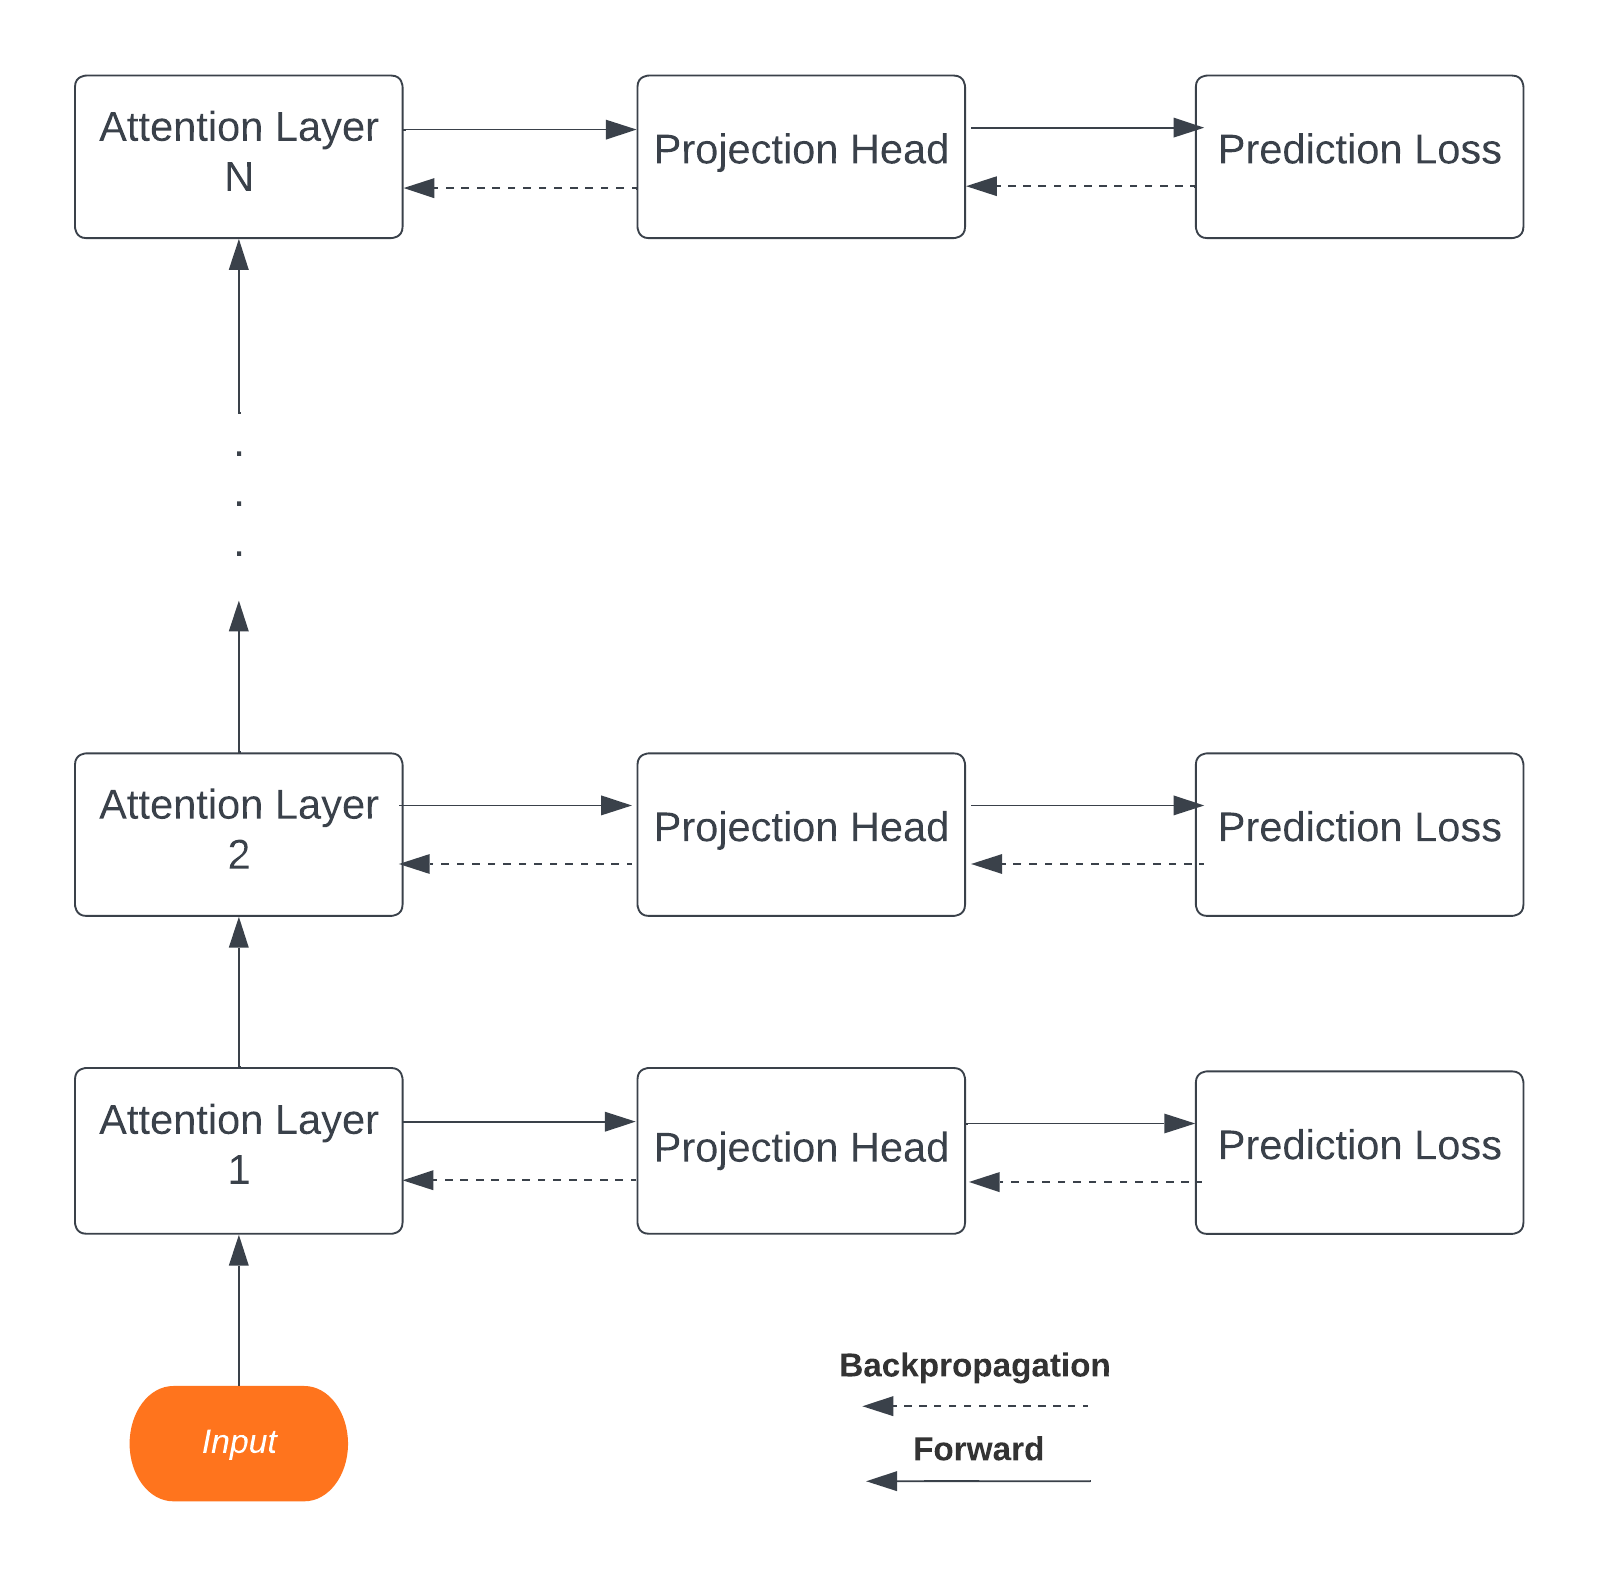
\includegraphics[width=8cm]{per layer training.png}}}%
	\caption{Per-layer training. The output of each layer is fed to the projection head and the loss is computed on it. The losses are then summed to create the loss of a single training step.}
	\label{per-layer-training}
\end{figure*}

% \subsection{Tasks and Datasets}

% % [intro and statistics to 6 datasets]
% We compare ICL and finetuning based on six datasets spanning three classification tasks. 
% \textbf{SST-2}~\citep{sst}, \textbf{SST-5}~\citep{sst}, \textbf{MR}~\citep{mr} and \textbf{Subj}~\citep{subj} are four datasets for sentiment classification; 
% \textbf{AGNews}~\citep{dbpedia:agnews} is a topic classification dataset; 
% and \textbf{CB}~\citep{cb} is used for natural language inference. 
% The statistics of the validation examples and label types are summarized in Table~\ref{tab:dataset}. 

% \subsection{Experimental Settings}

% In our experiments, we use two GPT-like pretrained language models with 1.3B and 2.7B model parameters, respectively, which are released by fairseq\footnote{\url{https://github.com/facebookresearch/fairseq}}. 
% In the rest of this paper, we call them GPT 1.3B and GPT 2.7B for short. 
% All experiments are conducted on NVIDIA V100 GPUs with 32 GB memory. 

% For each task, we use the same template to format examples for Zero-Shot Learning~(ZSL), ICL, and finetuning. 
% Details of the templates used for each task are provided in Appendix~\ref{appendix:template}. 
% The answer prediction processes for ZSL and finetuning are the same with ICL as described in Section~\ref{sec:bg_icl}, except that they do not have demonstration examples. 

% For ICL, we fix the number of demonstration examples to 32 and tune the random seed for each task to find a set of demonstration examples that achieves the best validation performance. 
% For finetuning, we use the same demonstration examples for ICL as the training examples and use SGD as the optimizer. 
% For a fair comparison, we fine-tune the model for only one epoch and the 
% training examples are provided in the same order as demonstrated for ICL. 
% We tune the learning rate for finetuning and select the one that achieves the best validation performance. 
% Details of the search range and selected value for the random seeds and learning rates are shown in Appendix~\ref{appendix:hyper}. 
\subsection{Evaluation Metrics}

In the following sections we describe the evaluation metrics used to compare the behavior of ICL and finetuning.
To ensure an optimal comparison, we have adopted the identical metrics as introduced in \cite{dai2023gpt}:
We design three metrics to measure the similarity between ICL and finetuning at three different levels: the prediction level, the representation level, and the attention behavior level. 

\paragraph{Prediction Recall}

From the perspective of model prediction, models with similar behavior should have aligned predictions.
We measure the recall of correct ICL predictions to correct finetuning predictions.
Given a set of test examples, we count the subsets of examples correctly predicted by each model: $C_{\text{ZSL}}, C_{\text{ICL}}, C_{\text{FT}}$.
To compare the update each method induces to the model's prediction we subtract correct predictions made in the ZSL setting.
Finally we compute the \textbf{Rec2FTP} score as: $\frac{ \sizeof{ \left( C_{\text{ICL}} \cap C_{\text{FT}} \right) \setminus C_{\text{ZSL}} } }{ \sizeof{ C_{\text{FT}} \setminus C_{\text{ZSL}} } }$ .
A higher Rec2FTP score suggests that ICL covers more correct behavior of finetuning from the perspective of the model prediction.

%This measure is agnostic to the inner workings of the attention mechanism.

\paragraph{Attention Output Direction}
In the context of an attention layer's hidden state representation space within a model, we analyze the modifications made to the attention output representation (\textbf{SimAOU}).

For a given query example, let $h^{(l)}_X$ represent the normalized output representation of the last token at the $l$-th attention layer within setting $X$. The alterations introduced by ICL and finetuning in comparison to ZSL are denoted as $h^{(l)}_{ICL} - h^{(l)}_{ZSL}$ and $h^{(l)}{FT} - h^{(l)}_{ZSL}$, respectively. We calculate the cosine similarity between these two modifications to obtain SimAOU ($\Delta FT$) at the $l$-th layer. A higher SimAOU ($\Delta FT$) indicates that ICL is more inclined to adjust the attention output in the same direction as finetuning.
For the sake of comparison, we also compute a baseline metric known as SimAOU (Random $\Delta$), which measures the similarity between ICL updates and updates generated randomly.

\paragraph{Attention Map Similarity}
We use SimAM to measure the similarity between attention maps and query tokens for ICL and finetuning.
For a query example, let $m^{(l,h)}_X$ represent the attention weights before softmax in the $h$-th head of the $l$-th layer for setting $X$. In ICL, we focus solely on query token attention weights, excluding demonstration tokens. Initially, before finetuning, we compute the cosine similarity between $m^{(l,h)}_{ICL}$ and $m^{(l,h)}_{ZSL}$, averaging it across attention heads to obtain SimAM (Before Finetuning) for each layer.
Similarly, after finetuning, we calculate the cosine similarity between $m^{(l,h)}_{ICL}$ and $m^{(l,h)}_{FT}$ to obtain SimAM (After FT). A higher SimAM (After FT) relative to SimAM (Before FT) indicates that ICL's attention behavior aligns more with a finetuned model than a non-finetuned one.

\section{Results}
Due to limitation in compute resources, we ran all of the experiments with pretrained GPT model with 1.3 billion model parameters (GPT 1.3B), Hence all of the results described in this section are on that model
\begin{table*}[t]
	% \subfloat[original]{
	% 	\begin{tabular}{|l|r|r|r|r|r|r|r|}
	% 		\hline \textbf{Metric $\textbackslash$ Task} & SST2   & SST5   & MR    & Subj   & AGNews & CB     & Average \\
	% 		\hline Sim AUO Random                        & 0.0017 & 0.0029 & 0.001 & 0.0025 & 0.0021 & 0.0037 & 0.0023  \\
	% 		\hline Sim AUO FT                            & 0.1091 & 0.113  & 0.219 & 0.193  & 0.3053 & 0.2013 & 0.1901  \\
	% 		\hline SimAM Before FT                       & 0.5547 & 0.3914 & 0.398 & 0.378  & 0.1516 & 0.1524 & 0.3376  \\
	% 		\hline SimAM After FT                        & 0.585  & 0.4047 & 0.498 & 0.487  & 0.4944 & 0.1875 & 0.4427  \\
	% 		\hline
	% 	\end{tabular}
	% }
	% \quad
	% \subfloat[per-layer]{
	% 	\begin{tabular}{|l|r|r|r|r|r|r|r|r|}
	% 		\hline \textbf{Metric $\textbackslash$ Task} & SST2   & SST5   & MR     & Subj   & AGNews & CB     & Average \\
	% 		\hline Sim AUO Random                        & 0.0016 & 0.0025 & 0.0008 & 0.0022 & 0.0021 & 0.0037 & 0.0021  \\
	% 		\hline Sim AUO FT                            & 0.2297 & 0.1065 & 0.3299 & 0.3439 & 0.3213 & 0.3435 & 0.2791  \\
	% 		\hline SimAM Before FT                       & 0.5546 & 0.3913 & 0.3979 & 0.3786 & 0.1518 & 0.1524 & 0.3377  \\
	% 		\hline SimAM After FT                        & 0.5774 & 0.4039 & 0.2919 & 0.2844 & 0.1201 & 0.0293 & 0.2845  \\
	% 		\hline
	% 	\end{tabular}
	% }

	\centering
	\subfloat{
		\begin{tabular}{|l|r|r|r|r|r|r|r|}
			\hline \textbf{Metric $\textbackslash$ Task} & SST2   & SST5   & MR     & Subj   & AGNews & CB     & Average         \\
			\hline SimAOU Random                         & 0.0016 & 0.0025 & 0.0008 & 0.0022 & 0.0021 & 0.0037 & 0.0021          \\
			\hline SimAOU FT                             & 0.1091 & 0.113  & 0.219  & 0.193  & 0.3053 & 0.2013 & 0.1901          \\
			\hline SimAOU Per-Layer FT                   & 0.2297 & 0.1065 & 0.3299 & 0.3439 & 0.3213 & 0.3435 & \textbf{0.2791} \\
			\hline
		\end{tabular}
	}
	\quad
	\subfloat{
		\begin{tabular}{|l|r|r|r|r|r|r|r|}
			\hline \textbf{Metric $\textbackslash$ Task} & SST2   & SST5   & MR     & Subj   & AGNews & CB     & Average         \\
			\hline SimAM                                 & 0.5546 & 0.3913 & 0.3979 & 0.3786 & 0.1518 & 0.1524 & 0.3377          \\
			\hline SimAM FT                              & 0.585  & 0.4047 & 0.498  & 0.487  & 0.4944 & 0.1875 & \textbf{0.4427} \\
			\hline SimAM Per-Layer FT                    & 0.5774 & 0.4039 & 0.2919 & 0.2844 & 0.1201 & 0.0293 & 0.2845          \\
			\hline
		\end{tabular}
	}
	\caption{SimAOU and SimAM on all 6 datasets, comparing similarity between baseline metrics, standard finetuning and per-layer fine-tuning.}
	\label{tab:per_layer_metrics}
\end{table*}

\subsection{Per-Layer Training}
We recreate the experiments of \cite{dai2023gpt} using the per-layer training method.
The results are shown in Table~\ref{tab:per_layer_metrics}.
The SimAOU metric is higher for the per-layer training, but the SimAM metric is lower, and even lower than without fine-tuning for most tasks.

We hypothesize, at this point, that the reason for the lower SimAM metric is the gradient norm size.
The first layers of the model are now trained on a new objective, i.e their output is projected to the vocabulary space and the cross-entropy loss is computed on it instead of being passed for the next numerous layers.
Because of that, the gradient norm may be larger than the gradient norm of the standard training process.
We verify this hypothesis by measuring the norm of the gradients of each attention layer, during the standard training process and the per-layer training process.
The results are shown in Figure \ref{grad_norm}.

Following this finding, we attempt to apply gradient clipping to the per-layer training process with limited success.
We experiment with different clipping values for one task (Subj) and are able to improve the metrics for this task, see Table~\ref{tab:per_layer_clipping_metrics}.
Yet, we find that each task requires a different clipping value, and aim to find a more principled approach.
We attempt to clip the gradients by normalizing them to allow a maximum norm that is the norm measured in the standard fine-tuning, but this does not improve the results.


\begin{figure*}%
	\centering
	\subfloat{{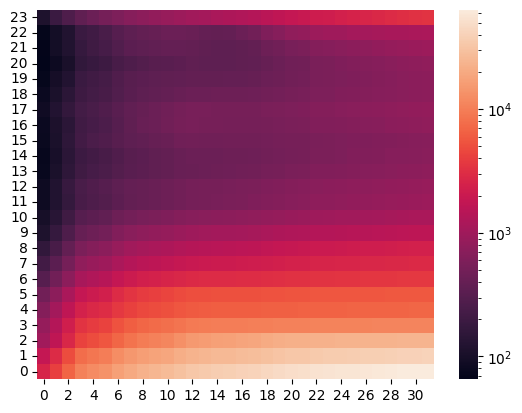
\includegraphics[width=6cm]{per_layer_grad_norm (1).png}}}%
	\subfloat{{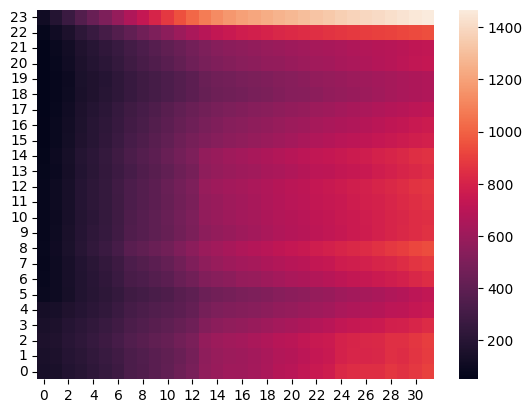
\includegraphics[width=6cm]{full_ft_grad_norm.png}}}%
	\caption{The gradient norm of each attention layer during the per-layer training process (left) and the standard fine-tuning process (right). The scale of the y-axis is different for each plot.}
	\label{grad_norm}
\end{figure*}


\begin{table*}[t]
	% \subfloat[Per-layer]{
	% 	\begin{tabular}{|l|r|r|r|r|r|r|r|}
	% 		\hline \textbf{Metric} & Subj   \\
	% 		\hline Sim AUO Random  & 0.0022 \\
	% 		\hline Sim AUO FT      & 0.3439 \\
	% 		\hline SimAM Before FT & 0.3786 \\
	% 		\hline SimAM After FT  & 0.2844  \\
	% 		\hline
	% 	\end{tabular}
	% }
	% \quad
	\centering
	\subfloat{
		\begin{tabular}{|l|r|}
			\hline \textbf{Metric $\textbackslash$ Task} & Subj   \\
			\hline Sim AUO Random                        & 0.0022 \\
			\hline Sim AUO FT                            & 0.348  \\
			\hline SimAM                                 & 0.3786 \\
			\hline SimAM After FT                        & 0.4227 \\
			\hline
		\end{tabular}
	}
	% \quad
	% \subfloat[Standard fine-tuning]{
	% 	\begin{tabular}{|l|r|}
	% 		\hline \textbf{Metric} & Subj   \\
	% 		\hline Sim AUO Random  & 0.0022 \\
	% 		\hline Sim AUO FT      & 0.193 \\
	% 		\hline SimAM Before FT & 0.3786 \\
	% 		\hline SimAM After FT  & 0.487 \\
	% 		\hline
	% 	\end{tabular}
	% }
	\caption{
		% Left shows the results for the per-layer training process. Middle shows the results for the per-layer training process with gradient norm clipping. Right shows the results for the standard fine-tuning process.
		Results for the per-layer training process with gradient norm clipping of max norm equal to 12.0.
		Compared to the results in Table~\ref{tab:per_layer_metrics}, the SimAM metric is higher than without the clipping, but not higher the standard fine-tuning process.
	}
	\label{tab:per_layer_clipping_metrics}
\end{table*}

% We first show the validation accuracy in the ZSL, ICL, and finetuning settings on six classification datasets in Table~\ref{tab:acc}. 
% Compared with ZSL, ICL and finetuning both achieve considerable improvements, which means the optimizations they make are both helpful to these downstream tasks. 
% In addition, we find that ICL is better at few-shot scenarios than finetuning. 

% \paragraph{Rec2FTP}
% We show the Rec2FTP scores for two GPT models on six datasets in Table~\ref{tab:similarity}. 
% As shown in the table, on average, ICL can correctly predict 87.64\% of the examples that finetuning can correct from ZSL. 
% These results indicate that at the prediction level, ICL can cover most of the correct behavior of finetuning. 

% \paragraph{SimAOU}
% We present the SimAOU scores averaged across examples and layers for two GPT models on six datasets in Table~\ref{tab:similarity}. 
% For comparison, we also provide a baseline metric~(\textbf{\textit{Random SimAOU}}) that computes the similarity between ICL updates and randomly generated updates. 
% From the table, we find that ICL updates are much more similar to finetuning updates than to random updates, which means at the representation level, ICL tends to change the attention results in the same direction as finetuning changes. 

% \paragraph{SimAM}
% Table~\ref{tab:similarity} also demonstrates the SimAM scores averaged across examples and layers for two GPT models on six datasets. 
% As a baseline metric for SimAM, \textbf{\textit{ZSL SimAM}} computes the similarity between ICL attention weights and ZSL attention weights. 
% Comparing these two metrics, we also observe that compared with ZSL, ICL is more inclined to generate attention weights similar to those of finetuning. 
% Again, at the attention behavior level, we prove that ICL behaves similarly to finetuning. 
\subsection{Linearization}
\begin{table*}[t]
	\centering
	\caption{SimAOU and SimAM on four datasets, comparing similarity between random and finetune for both original model and liniarization of the model.}
	\label{tabel:lin_results}
	\begin{tabular}{|l|cccc|c|}
		\hline
		Data \& Metric      & SST2   & SST5   & MR     & Subj  & Average        \\ \hline
		SimAOU Random       & 0.001  & 0.002  & 0.001  & 0.002 & 0.002          \\
		SimAOU FT           & 0.1091 & 0.113  & 0.219  & 0.193 & \textbf{0.158} \\
		SimAOU Lin Random   & 0.001  & 0.002  & 0.0007 & 0.002 & 0.001          \\
		SimAOU Lin FT       & 0.122  & 0.0789 & 0.171  & 0.148 & 0.130          \\ \hline
		SimAM Before FT     & 0.5547 & 0.3914 & 0.398  & 0.378 & 0.430          \\
		SimAM After FT      & 0.585  & 0.404  & 0.498  & 0.487 & \textbf{0.493} \\
		SimAM Lin Before FT & 0.554  & 0.391  & 0.397  & 0.378 & 0.4305         \\
		SimAM Lin After FT  & 0.573  & 0.403  & 0.448  & 0.449 & 0.468          \\ \hline
	\end{tabular}
\end{table*}

We calculated SimAOU and SimAM for both original and linearized models. Results are shown in Table \ref{tabel:lin_results}.
Due to limitation in compute resources, we ran all the experiment with pretrained GPT model with 1.3 billion model parameters (GPT 1.3B). In addition we were unable evaluate the linearized model on the datasets AGNews and CB due to heavy memory consumption. It is worth mentioning that we were able to replicate the results of GPT 1.3B from \cite{dai2023gpt} with a negligible difference.
The results indicate that the linearized model yields lower similarity scores compared to the original model but significantly higher scores than a random vector. This suggests that our hypothesis was incorrect and other simple model versions should be thought of. More on that in the discussion section.

\section{Discussions}
\subsection{Existence of an optimization process similar to ICL}
The mathematical analysis in Section~\ref{sec:icl_dual} suggests a similarity between ICL and finetuning.
Yet, it's important to note its limitations: (1) it is done on a linear attention layer (2) it is done on a single layer
(3) It is unclear what is the loss function for the optimization process that it suggests.
This means that the analysis is not sufficient to prove that non-linear, full model ICL is indeed a form of finetuning;
Hence, whether such an optimization process (or any kind of process) exists is still an open question.

\section{Related Work}

\section{Conclusion}
Following recent research that suggested a theoretical equivalency between in-context learning (ICL) and gradient descent (GD)-based fine-tuning, we've attempted to further explore this relationship in practical settings.
We experimented with a new training process that we call per-layer training,
and provided some empricial evidence to suggest that this process may explain the underlying mechanism of ICL better than standard fine-tuning.
Another experiment that we try is to fine-tune the model with linear approximation of it.
In our discussion section we discuss the limitations of our experiments, we also suggest that whether an optimization process similar to ICL exists is still an open question.
\section{Acknowledgement}
We would like to express appreciation to Guy Dar who supervised this project, for his help with formulating the research question and methodology, give insights and continuous feedback.

\bibliography{anthology,refs}
\bibliographystyle{acl_natbib}

\newpage
\appendix


\end{document}
